\section{Class M2: longer forward runs}\label{sec:mixed}

A period of class $\cls{M2}$ has switches of both signs, every maximal reverse run has exactly two
switches, and some maximal forward run has at least two (\cref{def:classes}). Unlike the classes
$\cls{R}$, $\cls{F}$ and $\cls{M1}$, such a period has no rigid sign word: the forward runs may
have any lengths, the number of reverse runs is arbitrary, and the factors are unrelated. The
exclusion uses a window of at most seven consecutive pieces around a smallest active margin.
Expressing the period's normal multiplier $U$ in this window gives a finite system of scalar
necessary conditions. We prove that this system is inconsistent. The whole period enters only
through three inputs: the compact domain (\cref{thm:compact-domain}), the cap on the Casimir that
competitiveness imposes, and a lower bound on the Casimir obtained from the winding of the switch
vectors over the period.

We prove \cref{thm:class-M2}.

The proof has five steps.
\begin{enumerate}[label=(\arabic*)]
\item A global minimum of the active margins occurs at the centre of a reverse run
(\cref{prop:m2-centre}).
\item Of the two turns beside that centre, choose the one with the smaller active margin; after
reflecting the period and reversing time if necessary, it follows the centre
(\cref{lem:m2-reflection}).
\item The switch after the chosen turn is forward or reverse. If it is reverse, the forward run
through the turn has a single switch (it is short), and \cref{sec:smaller-short} excludes the
window (\cref{thm:m2-smaller-short}). If it is forward, the run is nonshort, and the switch after
the next piece is again forward or reverse (\cref{prop:m2-window,prop:m2-continuation}).
\item A comparison that moves one margin to a boundary value turns the window into one scalar
residual $N$ that must be negative (\cref{lem:m2-comparison}), together with a short list of
necessary bounds (\cref{lem:m2-necessary}).
\item A reverse successor contradicts $N<0$ directly (\cref{thm:m2-reverse}). A forward successor
leaves a small region of parameters on which the Casimir of the period exceeds the competitive cap
(\cref{thm:m2-forward}).
\end{enumerate}
The first subsection carries out steps (1), (2), (4), (5) and the nonshort half of (3). The polynomial
inequalities are collected in \cref{app:nonshort-estimates}. Throughout, $\gamma^2$ is the Casimir of
\cref{def:normal-multiplier}, and the switch norms and turn secants are those of
\cref{lem:switch-norms}.

\subsection{The minimum and the nonshort continuations}\label{app:m2-nonshort}

\subsubsection{Three inputs from the whole period}\label{sec:m2-inputs}

Class $\cls{M2}$ requires a sharper cap than \cref{cor:casimir-cap}. We use the spectral form of
the cost--Casimir inequality, whose pointwise proof \eqref{eq:fwd-spectral-pointwise} applies
whenever the primary costate is negative elliptic.

\begin{lemma}[Casimir bounds]\label{lem:m2-casimir}
Let $P$ be a normal vertex period with cost $\cost$ and primary costate $\Lambda_1$.
\begin{enumerate}[label=(\alph*)]
\item If $\det\Lambda_1(0)>0$ and $\Lambda_1(0)_{10}<0$, then
$\cost\ge\frac\pi3\bigl(\kappa+\frac32\bigr)$ with $\kappa=\sqrt{\det\Lambda_1(0)}$.
\item If $P$ is competitive, then $\gamma^2<9193/50000$.
\item If $P$ is competitive and mixed, then $\gamma^2>27/256$.
\end{enumerate}
\end{lemma}

\begin{proof}[Sketch]
(a) Write $\Lambda_1(0)=-\kappa\,hJh^{-1}$ and $B=h^{-1}g$. The maximum condition gives pointwise
$2\kappa m_s\le 3m_b$, where $m_b=-\frac12\tr(JX)$ is a third of the cost density and
$m_s=-\frac12\tr(JBXB^{-1})$. The argument $\theta$ of $(B_{00}+B_{11})+i(B_{10}-B_{01})$ has
$\theta'=(m_b+m_s)/(z+1)$ with $z=\frac12\norm{B}_F^2\ge1$, and $g(T)=R$ forces
$\Delta\theta\ge\pi/3$. Since $\abs{z_B}^2=(z+1)/2$, \eqref{eq:fwd-spectral-key} is
$(m_b+m_s)^2\le2(z+1)m_bm_s$. Hence
$\theta'\le2m_bm_s/(m_b+m_s)\le6m_b/(2\kappa+3)$, and integration gives (a).
(b) Class $\cls{R}$ is impossible (\cref{thm:class-R}), so some switch is forward and has positive
norm; when $\gamma^2>0$, $\Lambda_1(0)$ is then negative elliptic (\cref{prop:ellipticity}), and
(a) with $\cost\le\Aoct$ gives $\kappa\le3\Aoct/\pi-3/2$.
The cost comparison of \cref{lem:octagon-cost-comparison} and the calculation in
\cref{cor:fwd-cap} then give $\gamma^2<9193/50000$.
(c) If $\gamma^2\le 27/256$, the Gram identity (\cref{lem:gram}) with $d_\pm\ge3/32$ puts the angle
between consecutive switch vectors below $\pi/3$ at a forward piece, and above $2\pi/3$ at a reverse
centre, by the angle gap $\cos\varphi<3/10$ of \cref{sec:short-runs}; a turn
contributes nothing. The increments then add up to more than $\pi/3$, while the winding of the switch
vectors over one period is exactly $\pi/3$ (\cref{sec:short-runs}).
\end{proof}

At a reverse centre (the middle piece of a reverse run of two) the pairing and the Casimir are
explicit functions of four quantities. With active margin $a$, turn neighbours $p,n$ and incident
norms $u_{\mathrm i},u_{\mathrm o}$ (eight times the switch norms, which are turn secants), put
$r=a/(a+p)$, $t=a/(a+n)$ and $\rho=a^2/(a^2+4)$. Stationarity at the centre and the Gram identity
read
\begin{equation}\label{eq:m2-centre}
\gamma^2=\frac{4u_{\mathrm i}u_{\mathrm o}-E^2}{16(1-\rho)^2},\qquad
E=1+r+t-\rho+\log\frac{\rho}{rt}-\frac{1-u_{\mathrm i}}{r}-\frac{1-u_{\mathrm o}}{t}.
\end{equation}
The strict centre minimum gives $r,t<\frac12$, and the positive reverse factor gives $\rho<rt$.

\begin{lemma}[Scale of a reverse centre]\label{lem:m2-scale}
In a competitive mixed normal vertex period, every reverse centre has active margin $a$ with
$a^2<12/17$.
\end{lemma}

\begin{proof}
The bound is $\rho<3/20$. Lowering both incident norms to their common floor $3/4$, and then raising
both ratios $r,t$ to $\frac12$, only decreases the right side of \eqref{eq:m2-centre}, and gives
$\gamma^2>G(\rho)=(9/4-B(\rho)^2)/(16(1-\rho)^2)$ with $B(\rho)=1-\rho+\log(4\rho)$. The function
$G$ increases on $[3/20,1/4)$ and $G(3/20)>23/125>9193/50000$, which contradicts
\cref{lem:m2-casimir}(b) when $\rho\ge3/20$; and $\rho<rt<1/4$ always.
\Cref{fig:m2-domains}(a) shows $G$.
\end{proof}

\begin{figure}[tb]
\centering
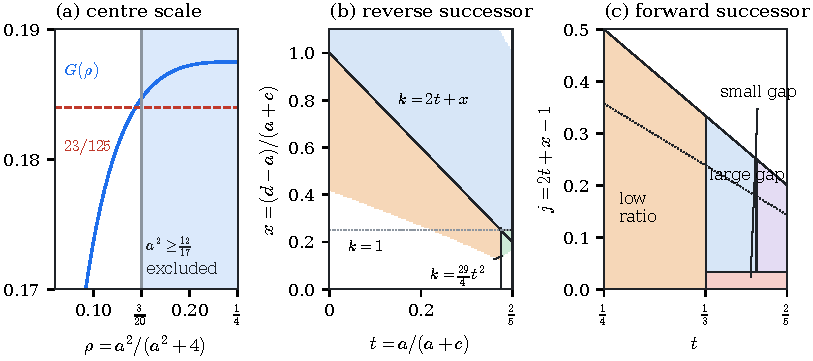
\includegraphics[width=\textwidth]{figures/fig-mixed-domains.pdf}
\caption{Parameter bounds for class $\cls{M2}$. (a)~The lower bound
$G(\rho)=(9/4-B(\rho)^2)/(16(1-\rho)^2)$ for the Casimir at a reverse centre, with
$\rho=a^2/(a^2+4)$. It exceeds the cap $23/125$ (dashed) on $[3/20,1/4)$, which proves
$a^2<12/17$ (\cref{lem:m2-scale}).
(b)~The parameters $(t,x)$ of the scalar reverse exclusion (\cref{prop:m2-reverse-core}), below
$x=1.1$, by the face to which $k$ is lowered: the unit shape $k=1$, the order face $k=2t+x$, and
the scale strip $k=29t^2/4$, which lies in $13/35<t<2/5$, $x\le9/35$. Points above $x=1$ belong to
the order face. (c)~The parameters $(t,j)$ of a forward successor, in $1/4<t<2/5$, $0<j<1-2t$: the
low ratio $t\le1/3$, the two large-gap regions $j\ge1/30$, split at $t=3/8$, and the small-gap
region, where the Casimir exceeds the cap. The dotted line is $j=\frac57(1-2t)$.}\label{fig:m2-domains}
\end{figure}

\subsubsection{The minimum is a reverse centre}\label{sec:m2-centre}

\begin{proposition}[The minimum is a reverse centre]\label{prop:m2-centre}
Let $P$ be a competitive normal vertex period of class $\cls{M2}$ with at least six pieces. There is
an index $m$ with $a_m\le a_k$ for every $k$ such that the switches $m-1$ and $m$ are reverse and the
switches $m-2$ and $m+1$ are forward.
\end{proposition}

Let $a_m$ be a smallest active margin of the period; the active margins are periodic, so a minimum
exists. A minimum cannot be at a turn: at three pieces with labels $i,j,i$ the active margins are
strictly log-concave, $a_{k}a_{k+2}<a_{k+1}^2$ (\cref{lem:three-arc}), so the middle one is not the
smallest of the three. If both switches at $m$ are reverse, $m$ is the centre of a reverse run. The
remaining case, both switches forward, is excluded by the following theorem, which uses only
stationarity and the floors that the two missing controls impose.

\begin{proposition}[No small forward minimum]\label{prop:m2-small-forward}
Let $P$ be a normal vertex period with at least three pieces, and let $m$ be an index such that the
switches $m-2,m-1,m,m+1$ are forward, $a_m\le a_j$ for $m-2\le j\le m+2$, and $a_m^2\le4/3$. This is
impossible.
\end{proposition}

The proof writes the multiplier in the frame of
the central piece, eliminates one coordinate with stationarity at the centre, and keeps the
stationarity row at the smaller neighbour with the two exterior floors $v\ge F_x(q)$ at the forward
switches. The remaining face is a one-variable residual with an exactly controlled second
derivative; two integrations and the Pad\'e bound $\frac12(h-h^{-1})-\log h\ge (h-1)^3/(3h(h+1))$
leave a rational expression, negative by an elementary cubic comparison. No Casimir bound is used.

\begin{proof}[Proof of \cref{prop:m2-centre}]
Take a global minimum $m$. If exactly one of the switches $m-1,m$ is reverse, the pieces $m-1,m,m+1$
have labels $i,j,i$, and \cref{lem:three-arc} contradicts minimality. If both are forward, the
strict centre minimum of the neighbouring reverse runs (\cref{prop:run-structure}) forces the
switches $m-2$ and $m+1$ to be forward as well: otherwise the centre of the adjacent reverse run
would have a smaller active margin. The period is mixed, so it has a reverse centre; by
\cref{lem:m2-scale} its active margin squared is below $12/17$, hence $a_m^2<12/17<4/3$, and
\cref{prop:m2-small-forward} gives a contradiction. If both switches are reverse, they form a
maximal reverse run, of length two in class $\cls{M2}$, and $m$ is its centre.
\end{proof}

\subsubsection{Orientation by reflection}\label{sec:m2-reflection}

Let $S=\mathrm{diag}(1,-1)$. Reflecting the plane and reversing time is a symmetry of the control
problem: it maps a normal vertex period to another one with the same cost, and reverses the order of
the pieces.

\begin{lemma}[Reflection]\label{lem:m2-reflection}
For every normal vertex period $P$ there is a normal vertex period $P'$ with the same number of
pieces and the same cost, whose state stays in $\hstarstar$ when that of $P$ does, with labels
$i'_k=c-i_{-1-k}$ for a constant $c\in\Z/3$ and active margins $a'_k=a_{-1-k}$. Its switch $k$ is
forward if and only if the switch $-2-k$ of $P$ is forward, and $P'$ is of class $\cls{M2}$ when $P$
is.
\end{lemma}

The construction is $u'(t)=\varsigma u(T-t)$, with $\varsigma$ the permutation of the vertices that
reflects the labels, $g'(t)=SR^{-1}g(T-t)S$, $X'(t)=-SX(T-t)S$, and $\Lambda'(t)=-S\Lambda(T-t)S$ for
both costates. Since $SJS=-J$, the cost density is preserved, and $\hstarstar$ is symmetric under
$x\mapsto-x$. Reading the signs in reverse order does not negate them: a reverse switch of $P$
is a reverse switch of $P'$.

By \cref{prop:m2-centre,lem:m2-reflection} we may assume that the global minimum $a=a_m$ is a
reverse centre and that the turn after it is the smaller one: $a_{m+1}\le a_{m-1}$. (At a tie either
choice works.) After relabeling the vertices by a power of $R$, which changes neither the cost nor
the active margins, the pieces $m-2,\dots,m+3$ have labels and active margins
\begin{equation}\label{eq:m2-labels}
0(p),\quad 1(b),\quad 0(a),\quad 2(c),\quad 0(d),\quad 1(r)
\end{equation}
when the switch $m+2$ is forward.
These are consecutive pieces of the period, continued through the twisted seam when necessary; they
need not be distinct from other pieces named later, and they are not a closed competitor.

\subsubsection{The nonshort window}\label{sec:m2-window}

\begin{table}[t]
\centering\small
\begin{tabular}{@{}l>{\raggedright\arraybackslash}p{0.74\textwidth}@{}}
\toprule
Symbol & Meaning (in \cref{sec:mixed} and \cref{app:nonshort-estimates})\\
\midrule
$p,b,a,c,d,r$ & active margins of six consecutive pieces \eqref{eq:m2-labels}; $a$ is a global
minimum, and $c\le b$\\
$K_a,\ Q,\ K_r$ & $a^2+4$, $d^2+4$, $r^2+4$\\
$S,T,W,Z,Y$ & $a+b$, $a+c$, $c+d$, $d+r$, $W^2-T^2$ (here $T$ is not the terminal time)\\
$u,v,w$ & eight times the norms of the switches $b\to a$; $a\to c$ and $c\to d$; $d\to r$\\
$h_a,h_d$ & the diagonal entries of the multiplier in the frames of the pieces $a$ and $d$\\
$U(x),\ g_B(x)$ & $1-x+x^2$ and $(B^2+Bx+x^2)/(B+x)^2=1-Bx/(B+x)^2$\\
$\operatorname{Sec}(A,B,P)$ & the average of $g_B$ over the interval between $A$ and $P$\\
$F_x(q)$ & $1+x^2q-xq\log q/(q-1)$, with $F_x(1)=U(x)$\\
$t,x,k,q$ & $a/T$, $(d-a)/T$, $K_a/T^2$, $WZ/Q$ (normalized coordinates)\\
$j$ & $2t+x-1$, the gap of a forward successor\\
\bottomrule
\end{tabular}
\caption{Local notation of class $\cls{M2}$. The letters $p,r,t,u,x$ have their usual meaning
elsewhere in the paper.}\label{tab:m2-notation}
\end{table}

\Cref{tab:m2-notation} lists the local notation. All quantities in the window come from the one
normal multiplier of the period. The factors of the same-sign pieces follow from the one-arc map
(\cref{lem:one-arc}) and the margins $(a_k,a_{k+1},(4-a_ka_{k+1})/(a_k+a_{k+1}))$ of the state at a
switch: the factor of a piece with incident signs $++$, $--$, $-+$, $+-$ is $s_{k-1}s_k/K_k$,
$K_k/(s_{k-1}s_k)$, $s_k/s_{k-1}$, $s_{k-1}/s_k$ respectively. In the window this gives
the central factor $K_a/(ST)>1$, the factor $q=WZ/Q>1$ of the piece $d$, and $d>a$ from the turn
$c$.

Both switches at a turn have the same norm, the turn secant (\cref{lem:switch-norms}):
$u=\operatorname{Sec}(a,b,p)$ and $v=\operatorname{Sec}(a,c,d)$, where
\[
\operatorname{Sec}(A,B,P)=1+\frac{B^2}{(A+B)(P+B)}-\frac{B}{P-A}\log\frac{P+B}{A+B}.
\]
In the frame of the central piece the multiplier is
\begin{equation}\label{eq:m2-Ua}
U_a=\begin{pmatrix}h_a&-K_a^2v/(8S^2)\\ S^2u/8&-h_a\end{pmatrix},\qquad
\gamma^2=\det U_a=\frac{uvK_a^2}{64}-h_a^2,
\end{equation}
and stationarity at the centre (\cref{lem:stationarity}) fixes the diagonal:
\begin{equation}\label{eq:m2-ha}
\begin{gathered}
h_a=\frac{K_a}{16a}\bigl(Su+Tv-C(b,a,c)\bigr),\\
C(p,a,n)=p+a+n-\frac{a^2}{p+a}-\frac{a^2}{a+n}+\frac{a^3}{a^2+4}
-a\log\frac{(p+a)(a+n)}{a^2+4}.
\end{gathered}
\end{equation}
Here $C(p,a,n)$ is four times the partial derivative of the normalized cost $\cost/\sqrt{12}$ in
the active margin of a same-sign piece. Transport across the centre and the turn to the frame of
the piece $d$ gives
\begin{equation}\label{eq:m2-transport}
h_d=h_a+\frac{vY}{8},\qquad w=\frac{uK_a^2+16h_aY+vY^2}{Q^2},
\end{equation}
and stationarity at $d$, the first piece of the forward run after the turn, is the root equation
\begin{equation}\label{eq:m2-root}
R_d:=C(c,d,r)-Wv-Zw+\frac{16\,d\,h_d}{Q}=0.
\end{equation}

\begin{proposition}[The nonshort window]\label{prop:m2-window}
Let $P$ be competitive, with state in $\hstarstar$, of class $\cls{M2}$ and with at least six pieces;
let $m$ be as in \cref{prop:m2-centre} with $a_{m+1}\le a_{m-1}$, and let the switch $m+2$ be
forward. Then $(p,b,a,c,d,r)=(a_{m-2},\dots,a_{m+3})$, with $u,v,h_a,w$ as above, satisfy:
\begin{enumerate}[label=(\roman*)]
\item the order $a<b$, $a<c\le b$, $a<p$, $a<d$, $a\le r$;
\item strict star at the five switches, $pb,ab,ac,cd,dr<4$; the factors $ST<K_a$ and $Q<WZ$;
three-arc log-concavity $ad<c^2$;
\item the compact domain: $a\ge2/15$, $cd+\frac2{15}(c+d)\le4$, $dr+\frac2{15}(d+r)\le4$,
$d,r\le8$, and $a+c,\,c+d,\,d+r\ge\frac12$; and the scale bound $a^2<12/17$;
\item the turn secants $u=\operatorname{Sec}(a,b,p)$, $v=\operatorname{Sec}(a,c,d)$; the switching
inequalities $g_b(p)\le u\le g_b(a)$, $g_c(d)\le v\le g_c(a)$, $w\ge g_d(r)$; the missing-control
floors $v\ge F_{d/W}(q)$ and $w\ge F_{d/Z}(q)$;
\item the identities \eqref{eq:m2-ha}, \eqref{eq:m2-transport} and \eqref{eq:m2-root};
\item $27/256<uvK_a^2/64-h_a^2<9193/50000$.
\end{enumerate}
\end{proposition}

\begin{proof}[Sketch]
Each item is read off the costate cycle at the switches of the window: (i) from minimality, the
choice $c\le b$ and \cref{prop:run-structure}; (ii) from the margin transports (\cref{lem:one-arc});
(iii) from \cref{thm:compact-domain} at the switching times (every margin is at least $2/15$, and
$y\le9/2$ on $\hstarstar$ gives the pair sums and $d,r\le8$) and \cref{lem:m2-scale}; (iv) from
\cref{lem:switch-norms} and, for the floors, from $H_i\le0$ for the two controls missing at a forward
switch, written through stationarity, an identity algebraic in
$x$ that holds for every $x$; (v) from exact transports; (vi) from \cref{lem:m2-casimir}.
\end{proof}

\subsubsection{The successor of the forward piece}\label{sec:m2-continuation}

The window does not yet contain a contradiction: the root equation \eqref{eq:m2-root} has solutions
compatible with (i)--(vi). The next actual switch, after the piece $r$, supplies one more condition.
Finiteness of the representation guarantees that it exists, and equal neighbouring labels have
been merged, so it is forward or reverse. Let
\[
t_{\mathrm{next}}=\frac{Q^2v-16h_dZ^2+wZ^4}{K_r^2}
\]
be the norm of that switch when it is forward, read in the frame of the piece $r$.

\begin{proposition}[The continuation alternative]\label{prop:m2-continuation}
In the situation of \cref{prop:m2-window}:
\begin{enumerate}[label=(\alph*)]
\item if the switch $m+3$ is forward, to a piece with active margin $s$, then $s\ge a$, $rs<4$,
$K_r<Z(r+s)$, $t_{\mathrm{next}}\ge g_r(s)\ge\frac34$, and both missing-control floors hold at the
piece $r$;
\item if the switch $m+3$ is reverse, to a piece with active margin $A$, then $a\le A<d$, $Ad<r^2$,
$w=\operatorname{Sec}(A,r,d)$ and $w\le g_r(A)$.
\end{enumerate}
\end{proposition}

In (a) the inequality for $t_{\mathrm{next}}$ is the forward switching inequality at the piece $r$,
whatever the margin $s$ and the length of the forward run. In (b) the piece $r$ is a turn, both its
switches have the norm $\operatorname{Sec}(A,r,d)$, $A\ge a$ by minimality, and $Ad<r^2$ is
three-arc log-concavity. Since $g_r$ decreases on $(0,r)$ and $A<r$, extending the average from
$[A,d]$ to $[a,d]$ also gives $w\le\operatorname{Sec}(a,r,d)$; we use (b) as stated.

\subsubsection{The boundary comparison and the residual}\label{sec:m2-comparison}

The root equation \eqref{eq:m2-root} is affine in the incident norm $u$, with slope
\begin{equation}\label{eq:m2-Ru}
\partial_uR_d=\frac{K_a}{aQ^2}\bigl(dSQ-Z(aK_a+SY)\bigr)<0,
\end{equation}
negative because $Y>0$, $Z>Q/W$, and $dSQ-Z(aK_a+SY)<(Q/W)\{a(ST-K_a)+Sc(a-d)\}<0$. The reverse
switch $b\to a$ caps $u$ by the ceiling $U(a/S)=g_b(a)$, so the actual data satisfy
$R_d(U(a/S))\le R_d(u)=0$. Stationarity at $d$ thus imposes an upper bound on the incident norm. On the necessary domain,
we will show that stationarity instead requires the norm to exceed this ceiling.

Before testing this, we remove the margins $b$ and $p$. Keep $a,c,d,r$ and the actual $v$ fixed and
raise $b$ to $b_*=K_a/T-a$, the value at which the central factor $K_a/(ST)$ equals one. Write
$G(b)=R_d(U(a/(a+b));b)$ for the residual at the ceiling, with $h_a$ given by central stationarity at
the margin $b$.

\begin{lemma}[Boundary comparison]\label{lem:m2-comparison}
For the window of \cref{prop:m2-window}, $G(b_*)<0$; the root $u_*$ of $R_d(\,\cdot\,;b_*)=0$
satisfies $u_*<U(aT/K_a)$; and the outgoing norm $w_*$ of that boundary root satisfies $w_*<w$.
\end{lemma}

\begin{proof}
Along $[b,b_*]$ the derivative is $G'(b)=\partial_uR_d\cdot a(b-a)/(a+b)^3<0$, and at the actual
margin $G(b)=\partial_uR_d\,(U(a/S)-u)\le0$, so $G(b_*)<0$. Along the curve of roots $u(b)$, the
outgoing norm has $dw/db=dK_a^3G(b)/(aQ^3(\partial_uR_d)^2)<0$, so $w$ decreases from its actual
value.
\end{proof}

This is a scalar comparison: the point $b_*$ need not belong to a trajectory, and no switching
inequality, floor or Casimir bound is transported to it.

At $b_*$ the logarithm of the centre disappears ($C(b_*,a,c)=4/T+4c/K_a$), and homogeneity lets us
normalize by $T=a+c$. In the coordinates $t=a/T$, $x=(d-a)/T$, $k=K_a/T^2$, $q=WZ/Q$, write
$W=1+x$, $p=t+x$ and $B=k+2tx+x^2$ for the normalized values; the margins are recovered from
$(t,x,k,q)$, since $a^2(k-t^2)=4t^2$. The positive multiple
\[
N(t,x,k,q,v,\log q)=t\,B\,q\,W\cdot\frac{G(b_*)}{T}
\]
is a polynomial in $t,x,k,q,v$ and $L=\log q$, affine in $k$, in $v$ and in $L$; \cref{app:m2-residual} gives its coefficients. The normalized
incoming secant is $v=\operatorname{Sec}(t,1-t,t+x)=1+(1-t)^2/W-(1-t)\log W/x$.

\begin{lemma}[Shape monotonicity]\label{lem:m2-shape}
If $0<t<1$, $x>0$, $q\ge1$, $v\le U(t)$ and $L<q-1$, then $N(t,x,k,q,v,L)$ is nondecreasing in $k$.
\end{lemma}

The coefficient of $k$ is at least $q\,t\,x(1-t)\{(q-1)(2x+1)+tx\}>0$ (\cref{app:m2-residual}).
Since $k$ moves with $a$ at fixed $t$, the lemma lets every later argument lower $k$ to the smallest
value that the necessary conditions allow, and prove $N>0$ there.

\begin{lemma}[Necessary conditions]\label{lem:m2-necessary}
Every window of \cref{prop:m2-window} satisfies
\begin{enumerate}[label=(\roman*)]
\item $0<t<\frac12$, $x>0$, $k>1$, $1<q<W/p$, $v=\operatorname{Sec}(t,1-t,t+x)$,
$1-(1-t)p/W^2\le v\le U(t)$ and $F_{p/W}(q)\le v$;
\item $N(t,x,k,q,v,\log q)<0$;
\item $t<2/5$;
\item $a<4/5$, that is, $k>29t^2/4$;
\item $d^2+2cd>4$, that is, $k<2t+2x+x^2$;
\item $3d<7c$, that is, $x<\frac73-\frac{10}3t$;
\item if the successor is reverse, $d\le b_*$, that is, $k\ge2t+x$.
\end{enumerate}
\end{lemma}

Item (i) restates the window ($k>1$ is $ST<K_a$ with $S\ge T$, and $q<W/p$ is $dr<4$); the
others are proved in \cref{app:m2-bounds}.

\subsubsection{The reverse successor}\label{sec:m2-reverse}

\begin{proposition}[The scalar reverse exclusion]\label{prop:m2-reverse-core}
Let $0<t<2/5$, $x>0$, $\max\{1,\,2t+x,\,29t^2/4\}\le k<2t+2x+x^2$, $x<\frac73-\frac{10}3t$,
$1<q<(1+x)/(t+x)$, $v=\operatorname{Sec}(t,1-t,t+x)\le U(t)$ and $F_{(t+x)/(1+x)}(q)\le v$.
Then $N(t,x,k,q,v,\log q)>0$.
\end{proposition}

\begin{proof}
By \cref{lem:m2-shape} it suffices to find a shape $k'\le k$ allowed by the hypotheses with
$N(k')>0$. There are three exhaustive cases (\cref{fig:m2-domains}(b)).
\begin{enumerate}[label=(\arabic*)]
\item If $t\le13/35$ and $x\le1-2t$, lower $k$ to $1$, where $N(1)>0$ (\cref{lem:m2-unit-shape}).
\item If $2t+x\ge1$ and $x>1/4$, lower $k$ to the order face $k=2t+x$. The floor and the swapped
secant order give $q\le(1+x)/(2t+x)$. On this face $N$ is a positive
multiple of a function $\alpha+\beta q+\gamma/q-p\log q$, concave in $q$, so it suffices to check
$q=1$ and the upper end, where it is positive (\cref{lem:m2-order-face}).
\item Otherwise $13/35<t<2/5$ and $x\le9/35$; lower $k$ to the scale face $k=29t^2/4$, where
$N>0$ (\cref{lem:m2-strip}).\qedhere
\end{enumerate}
\end{proof}

On each face the logarithms are first replaced by rational bounds with the correct signs ($v$ by a
larger $\bar v$, $\log q$ by $L_+(q)\ge\log q$, the floor by a smaller $F_\ell$), which lowers $N$; the
result is a cubic in $y=q-1$ whose positivity for $y\ge0$ follows from six polynomial signs in
$(t,x)$. \Cref{app:m2-reverse-signs} gives the reduction and proves the signs.

\begin{theorem}[Reverse successor]\label{thm:m2-reverse}
No window of \cref{prop:m2-window} has a reverse successor.
\end{theorem}

\begin{proof}
By \cref{prop:m2-continuation}(b) and \cref{lem:m2-necessary}, the normalized window satisfies every
hypothesis of \cref{prop:m2-reverse-core}, which gives $N>0$, against \cref{lem:m2-necessary}(ii).
\end{proof}

\subsubsection{The forward successor}\label{sec:m2-forward}

When the successor is forward the order bound (vii) fails, and the residual alone does not suffice.
Two facts replace it. First, the scalar reverse exclusion applies to every window with $k\ge2t+x$,
without any assumption on the successor, so every window has the opposite order
\begin{equation}\label{eq:m2-order}
k<2t+x,\qquad\text{equivalently } d>b_*\text{ and } j=2t+x-1>0.
\end{equation}
Second, the forward successor gives a lower bound for the next norm at the
boundary root. Both the actual point and the boundary point satisfy the root equation
\eqref{eq:m2-root}, which makes $h_d$ an affine function of $w$; on that line the next norm is a
decreasing affine function of $w$, and $w_*<w$, so the next norm $t_{\mathrm{next},*}$ at the
boundary is at least $t_{\mathrm{next}}\ge\frac34$. As a function of the
incident norm the next norm is affine, and its value at the root differs from its value
$\mathcal T_U$ at the ceiling by a multiple of $N$. For multipliers $\alpha>0$ and $M\ge0$ the
combined residual
\begin{equation}\label{eq:m2-comb}
\begin{aligned}
\mathcal H&=\alpha N+C_*\bigl(\tfrac34-t_{\mathrm{next},*}\bigr)+M\bigl(F_{p/W}(q)-v\bigr)\\
&=(\alpha+1-Je^2)N+C_*\bigl(\tfrac34-\mathcal T_U\bigr)+M\bigl(F_{p/W}(q)-v\bigr),
\end{aligned}
\end{equation}
with $e=q/W$, $J=t+x(x+2)$ and an explicit $C_*>0$, is therefore negative at every window with a
forward successor. It is affine in $v$, in $\log q$ and in the floor value,
and a concave quadratic in $k$.

The unit face of the low-scale argument gives $t>1/4$ (\cref{lem:m2-low-unit}); with the
derivative floor $v\ge g_c(d)$ this gives $x<1$ and $4t+x<2$, and a quantitative form of the swapped
secant order gives $q<W/(1+2j)$. The remaining parameters are cut down in
three steps (\cref{fig:m2-domains}(c)).

\begin{proposition}[The forward successor in three steps]\label{prop:m2-forward-steps}
Every window of \cref{prop:m2-window} with a forward successor satisfies
\begin{enumerate}[label=(\alph*)]
\item $t>1/3$;
\item $j=2t+x-1<1/30$;
\end{enumerate}
and then the Casimir of the period is at least $9193/50000$, against \cref{lem:m2-casimir}(b).
\end{proposition}

\begin{proof}[Outline]
(a) If $t\le1/3$, take $\alpha=6$ and $M=0$. The coefficients of $v$ and of $\log q$ in $\mathcal H$
are negative, so raising $v$ to a rational majorant $\hat v$ and $\log q$ to $L_+(q)$ keeps
$\mathcal H$ negative. The result increases in $k$, so it is negative at $k=1$ as well; but at
$k=1$ it is positive (\cref{lem:m2-low-ratio}).

(b) Suppose $j\ge1/30$. Then $1/3<t<2/5$ by (a), and the derivative floor in integral form gives
$j<\frac57(1-2t)$. For $1/3\le t\le3/8$ take $\alpha=\frac72-10(q-1)$ and $M=8j+8(q-1)-\frac16$,
both positive here; after the substitutions of $v$, $\log q$ and the floor by rational bounds, the
residual increases in $k$ and is positive at $k=1$. For $3/8\le t<2/5$ take $\alpha=4$ and $M=1$;
the residual increases in $k$ and is positive at the scale face $k=29t^2/4$
(\cref{lem:m2-large-gap}).

(c) Now $1/3<t<2/5$, $0<j<1/30$ and $1\le k<31/30$. With $N<0$, a rational comparison in $q$ gives
$\chi=pq/W>4/7$ (\cref{lem:m2-chi}). On the stationarity line of the piece $d$, the diagonal $h_d$
is an affine function $H_d(w)$ of the outgoing norm, and the Casimir is
$\Gamma(w)=(4B^2vw-H_d(w)^2)/(16(k-t^2)^2)$ in normalized form. For
$w\ge3/4$ one has $\Gamma'(w)<0$ (\cref{lem:m2-slope}). The actual $w$ lies between $3/4$ and the
central upper envelope $w_U$, the transported norm with $u$ at its ceiling and $b=b_*$, so $\gamma^2=\Gamma(w)>\Gamma(w_U)$. At $w_U$ the event factor $q$ is
eliminated with the floor (\cref{lem:m2-qelim}), and the remaining function of $(t,x,k,v)$
exceeds $9193/50000$ (\cref{lem:m2-envelope}).
\end{proof}

\begin{theorem}[Forward successor]\label{thm:m2-forward}
No window of \cref{prop:m2-window} has a forward successor.
\end{theorem}

This is \cref{prop:m2-forward-steps}. The obstruction in its last step is the cost itself: the turn
data force the Casimir of the period above $9193/50000$, and by \cref{lem:m2-casimir}(a) a period
with such a Casimir costs more than $\Aoct$.

\begin{remark}[Small scale]\label{rem:m2-low-scale}
The same methods exclude every window with $a\le\frac12$, whatever the sign of the successor:
then $k\ge17t^2$, and
$N$ can be lowered to $k=1$ or to $k=2t+\frac12$. The proof above needs only the unit face of that
argument (\cref{lem:m2-low-unit}), which gives $t>1/4$.
\end{remark}


\subsubsection{Proof of \texorpdfstring{\cref{thm:class-M2}}{the theorem for class M2}}\label{sec:m2-proof}

Let $P$ be as in \cref{thm:class-M2}, and take $m$ from \cref{prop:m2-centre}. If $a_{m+1}>a_{m-1}$,
replace $P$ by its reflection (\cref{lem:m2-reflection}): it is again competitive, of class
$\cls{M2}$, with state in $\hstarstar$ and the same number of pieces; the minimum moves to $-1-m$,
the four switches around it keep their signs in reverse order, and the smaller turn now follows the
centre. If the switch $m+2$ after the turn is reverse, the seven pieces $m-2,\dots,m+4$ form a
smaller-short window, excluded by \cref{thm:m2-smaller-short}. If it is forward, \cref{prop:m2-window} gives a nonshort window,
and \cref{prop:m2-continuation} gives a forward or a reverse successor; \cref{thm:m2-forward}
and \cref{thm:m2-reverse} exclude them. \qed

\subsection{Estimates for class M2: the nonshort cases}\label{app:nonshort-estimates}

This subsection proves the scalar inequalities behind \cref{sec:mixed}, in the notation of
\cref{tab:m2-notation}. Every step concerns explicit functions of at most five real variables.
The logarithm estimates follow from one reciprocal integral, using Jensen's inequality and
pointwise bounds on the integrand. They give bounds for the secants and the duration. The
remaining face arguments reduce polynomial signs, one variable at a time, to inequalities on
intervals. Several of these polynomials are long; they are determined by the displayed
definitions, and we state the identities and bounds on which each sign rests.

\subsubsection{Secants and floors}\label{app:m2-secants}

For $B>0$ the function $g_B(x)=1-Bx/(B+x)^2$ decreases on $(0,B)$, increases on $(B,\infty)$, and
has minimum $g_B(B)=3/4$; also $g_B(x)=U(B/(B+x))=U(x/(B+x))$. The turn secant
$\operatorname{Sec}(A,B,P)=(P-A)^{-1}\int_A^Pg_B$ has the antiderivative
$s-B\log(B+s)-B^2/(B+s)$.

\begin{lemma}[Secants]\label{lem:m2-secants}
\begin{enumerate}[label=(\alph*)]
\item If $0<a\le c<d$, then $\operatorname{Sec}(a,c,d)<\operatorname{Sec}(a,d,c)$.
\item If $0<c\le d$, then $z\mapsto\operatorname{Sec}(z,d,c)$ strictly decreases on $(0,c]$.
\item For $P,C>0$ and $q>1$, $F_{P/(P+C)}(q)=\operatorname{Sec}((P+C)/q-P,\,P,\,C)$. In particular
$F_{d/W}(q)=\operatorname{Sec}(B_0,d,c)$ with $B_0=(4-dr)/(d+r)$, the third margin at the switch
$d\to r$.
\item If $ad<c^2$, then $\operatorname{Sec}(a,c,d)<\frac12(g_c(a)+g_c(d))$.
\item If $0<A<P$, $B>0$ and $B/(A+B)\ge3/5$, then $\operatorname{Sec}(A,B,P)>\mu_*:=(2\sqrt{130}-4)/25$.
\end{enumerate}
\end{lemma}

\begin{proof}
(a) $\operatorname{Sec}(a,d,c)=\int_0^1g_1(u)\,d\theta$ and $\operatorname{Sec}(a,c,d)=\int_0^1g_1(v)\,d\theta$
with $u=(a+\theta(c-a))/d$ and $v=(a+\theta(d-a))/c$. Here $v>u$, $uv<1$, and
$g_1(u)-g_1(v)=(v-u)(1-uv)/((1+u)^2(1+v)^2)>0$.
(b) The derivative is $(\operatorname{Sec}(z,d,c)-g_d(z))/(c-z)$, and the average of the decreasing
function $g_d$ over $[z,c]$ is below its value at $z$.
(c) Substitute $(P+C)/q-P$ in the closed form of the secant; $W/q-d=Q/Z-d=B_0$.
(d) For $a\le x\le d$,
\begin{multline*}
\frac{(d-x)g_c(a)+(x-a)g_c(d)}{d-a}-g_c(x)\\
=\frac{c(x-a)(d-x)\,[c^2(a+d+2c)+(c^2-ad)x]}{(a+c)^2(d+c)^2(x+c)^2}\ge0;
\end{multline*}
integrate over $[a,d]$.
(e) With $\eta=B/(A+B)$ and $q=(P+B)/(A+B)>1$, the secant is
$1+\eta^2/q-\eta\log q/(q-1)$. The upper bound of \cref{lem:m2-logs}(b) gives
\[
 \operatorname{Sec}(A,B,P)>
 1-\frac\eta6+\frac{a}{q}-\frac{b}{q+1},\qquad
 a=\eta\left(\eta-\frac16\right),\quad b=\frac{4\eta}{3}.
\]
For $a,b>0$, completing a square gives
\[
 \frac{a}{q}-\frac{b}{q+1}+(\sqrt b-\sqrt a)^2
 =\frac{\bigl(\sqrt a(q+1)-\sqrt b\,q\bigr)^2}{q(q+1)}\ge0.
\]
Thus the secant exceeds
\[
 m(\eta)=1-\eta^2-\frac{4\eta}{3}+\frac{2\eta}{3}\sqrt{12\eta-2}.
\]
This lower bound increases on $1/2\le\eta\le1$. Indeed, with
$w=\sqrt{12\eta-2}-2$, it is $3/4+w^2(4-w^2)/144$, and $0\le w^2<2$ on that interval.
For $\eta\ge3/5$ we obtain
$\operatorname{Sec}(A,B,P)>m(3/5)=\mu_*$.
\end{proof}

\subsubsection{Rational bounds for the logarithms}\label{app:m2-logs}

\begin{lemma}[Logarithms]\label{lem:m2-logs}
Let $0<t<1$, $x>0$, $q>1$, $c=1-t$, $W=1+x$, $X=x+2$, $p=t+x$, $g=1-cp/W^2$, and let
$v=1+c^2/W-c\log W/x$ be the normalized incoming secant.
\begin{enumerate}[label=(\alph*)]
\item $\log(1+x)>2x/X+2x^3/(3X^3)$; hence $v<\bar v=1+c^2/W-(2c/X)(1+x^2/(3X^2))$.
\item $\log q<L_+(q)=(q-1)(q^2+10q+1)/(6q(q+1))$; hence
$F_{p/W}(q)>F_\ell=1+p^2q/W^2-(p/W)(q^2+10q+1)/(6(q+1))$.
\item With $\tau=x/X$,
$\log(1+x)>L_J(x):=2\tau\bigl(1+\tau^2/[3(1-3\tau^2/5)]\bigr)$; hence
$v<v_G=g+(cx/W^2)(T_G(x)-t)$ with $T_G=(90-19x^2)/(12(x^2+10x+15))$.
\item $\log(1+x)>3x(x+2)/(x^2+6x+6)$; hence $v<V=1+c^2/W-3c(x+2)/(x^2+6x+6)$.
\item $\bar v-g=((1-t)x/W^2)(T(x)-t)$ with $T(x)=(-2x^3-x^2+10x+12)/(3(x+2)^3)$; so $v\ge g$ forces
$t<T(x)$. The function $T$ decreases, and $T(1)=19/81<1/4$.
\end{enumerate}
\end{lemma}

\begin{proof}
All the logarithm bounds follow from the reciprocal integral
\[
 \log\frac{1+\tau}{1-\tau}=2\tau I(\tau),\qquad
 I(\tau)=\int_0^1\frac{\dd s}{1-\tau^2s^2}\qquad(0<\tau<1).
\]
For (a), the integrand exceeds $1+\tau^2s^2$. For (b), it is less than
$1+\tau^2s^2/(1-\tau^2)$ for $0<s<1$. Integration gives
$I(\tau)<1+\tau^2/[3(1-\tau^2)]$; at $\tau=(q-1)/(q+1)$ this is the displayed upper bound.

For (c), write
$I(\tau)=1+\tau^2\int_0^1s^2/(1-\tau^2s^2)\,\dd s$.
Apply strict Jensen to $y\mapsto(1-\tau^2y)^{-1}$ with probability density $3s^2$.
The mean of $s^2$ is $3/5$, giving $I(\tau)>1+\tau^2/[3(1-3\tau^2/5)]$.
As $c>0$, this implies $v<v_J:=1+c^2/W-cL_J(x)/x$. The required ceiling follows from
\[
 v_G-v_J=\frac{cx^6}{12W^2(x+2)(x^2+10x+10)(x^2+10x+15)}>0.
\]
For (d), Jensen with uniform measure gives $I(\tau)>1/(1-\tau^2/3)$.
The resulting logarithm bound also has the direct verification
\[
 \frac{\dd}{\dd x}\left(\log(1+x)-\frac{3x(x+2)}{x^2+6x+6}\right)
 =\frac{x^4}{(1+x)(x^2+6x+6)^2}>0;
\]
the difference vanishes at $x=0$. Part (e) follows by subtraction and
$T'(x)=-(11x^2+24x+16)/(3(x+2)^4)$.
\end{proof}

\subsubsection{The residual}\label{app:m2-residual}

Put $c=1-t$, $p=t+x$, $W=1+x$, $Y=x(x+2)$, $B=k+2tx+x^2$, $Z=qB/W$ (the normalized $d+r$), and
\[
H_0=\frac kt\,(v-1+t^2)+t(2-t),\qquad w_U=\frac{k^2-kt+t^2+H_0Y+vY^2}{B^2},
\]
the central diagonal and the transported outgoing norm with the incident norm at the boundary
ceiling $U(t/k)$. The root function at the ceiling, divided by $T$, is
\[
R=c+Z-\frac{p^2}{W}-\frac{p^2}{Z}+\frac{p^3}{B}-p\log q-Wv-Zw_U+\frac{p(H_0+2vY)}{B},
\]
and $N=tBqW\,R$. Clearing denominators cancels every negative power, and $N$ is a polynomial,
affine in $k$, $v$ and $L=\log q$:
\begin{itemize}
\item the coefficient of $v$ is $N_v=-xq\,I$ with
$I=k+tx+tW(k-2t)+(q-1)\bigl(kX+txX^2\bigr)$, nonpositive when $k\ge2t$;
\item the coefficient of $L$ is $N_L=-tpqWB\le0$;
\item the coefficient of $k$ is
\begin{multline*}
A=q\bigl\{x[(1-v)(1+tW)-t(1-t^2)]\\
+(q-1)[t^2(1+2x-x^2)+2tx^2+(1-v)Y]-tpW L\bigr\}.
\end{multline*}
\end{itemize}
In $A$ the coefficient of $v$ is $-qx[(q-1)(x+2)+1+tW]<0$ and that of $L$ is $-qtpW<0$. Inserting
$v\le U(t)=1-t+t^2$ and $L<q-1$ and collecting gives
$A>q\,t\,x(1-t)[(q-1)(2x+1)+tx]>0$, which is \cref{lem:m2-shape}.

\begin{lemma}[Rational relaxation]\label{lem:m2-relax}
If $k\ge2t$, $q>1$ and $F_{p/W}(q)\le v$, then
\[
N(v,\log q)\ \ge\ N(\bar v,L_+)-(q-1)(\bar v-F_\ell),
\]
and $P_k:=6(q+1)W^2X^3\{N(\bar v,L_+)-(q-1)(\bar v-F_\ell)\}$ is a polynomial in $t$, $x$, $k$ and
$y=q-1$, cubic in $y$.
\end{lemma}

\begin{proof}
$N_v\le0$, $N_L\le0$, $v<\bar v$ and $\log q<L_+$, while $F_\ell<F_{p/W}(q)\le v<\bar v$ makes the
subtracted term nonnegative.
\end{proof}

\subsubsection{The necessary bounds}\label{app:m2-bounds}

We prove \cref{lem:m2-necessary}(iii)--(vii).

\runin{The scale.} At the centre, \eqref{eq:m2-centre} holds with $u_{\mathrm i}=u$,
$u_{\mathrm o}=v$, $r=a/S$ and $t=a/T$. Lowering both norms to a floor $\mu$ and raising both ratios
to a cap $\zeta$ gives $\gamma^2\ge(4\mu^2-B(\rho)^2)/(16(1-\rho)^2)$ with
$B(\rho)=1-\rho+\log\rho+2\psi_\mu(\zeta)$, $\psi_\mu(\zeta)=\zeta-\log\zeta-(1-\mu)/\zeta$. The
cleared comparison $\varphi(\rho)=4\mu^2-B(\rho)^2-16\,\Gamma_{\max}(1-\rho)^2$, with
$\Gamma_{\max}=9193/50000$, has derivative $2(1-\rho)(16\Gamma_{\max}-B/\rho)$ and increases, so its
positivity at the left end of an interval of $\rho$ excludes that interval by
\cref{lem:m2-casimir}(b). With the floor $3/4$ and the cap $1/2$ this gives $a^2<2/3$, that is
$\rho<1/7$. When $t\le2/5$, both ratios are at most $2/5$ and both turns have middle-margin ratio
$B/(A+B)\ge3/5$, so \cref{lem:m2-secants}(e) gives the intrinsic floor $\mu=\mu_*$.
For completeness, put $\rho_0=4/29$, $\zeta=2/5$ and
\[
 B_* =1-\rho_0+2\zeta-\frac{2(1-\mu_*)}{\zeta}
       -\frac{2(\zeta^2-\rho_0)}{\zeta^2+\rho_0}.
\]
The elementary bound $\log y<y-1$ and $\mu_*>3/4$ give $B(\rho_0)>0$.
The symmetric reciprocal bound for $\log(\zeta^2/\rho_0)$ then gives
$B(\rho_0)<B_*$, and a squaring in $\sqrt{130}$ gives
\[
 4\mu_*^2-B_*^2-16\Gamma_{\max}(1-\rho_0)^2>0.
\]
Moreover $B$ increases, and the same logarithm bound, together with
$\mu_*<U(\zeta)$, gives $B(3/20)<16\Gamma_{\max}\rho_0$.
Thus $\varphi$ increases throughout $[\rho_0,3/20]$, whose left endpoint
is already positive. This excludes that interval and proves $a<4/5$.
In normalized form $a^2(k-t^2)=4t^2$, so $a^2<2/3$ is $k>7t^2$, and $a<4/5$
is $k>29t^2/4$.

\begin{samepage}
\begin{lemma}[The centre gap]\label{lem:m2-centre-gap}
Every window of \cref{prop:m2-window} has $d^2+2cd>4$,
or equivalently $k<2t+2x+x^2$ in normalized coordinates.
\end{lemma}

\begin{proof}
First raise the incident norm $u$ to its ceiling at the actual margin $b$,
and then raise $b$ to $b_*=K_a/T-a$.
The outgoing norm increases in $u$. For the second comparison put
$S=a+b$ and $S_*=a+b_*=K_a/T$. Since $2a<S<S_*$, the diagonal at the upper incident norm satisfies
\begin{align*}
 h_U(S_*)-h_U(S)
 &=\frac{K_a}{16}\left\{2a\left(\frac1{S_*}-\frac1S\right)-\log\frac S{S_*}\right\}\\
 &\ge\frac{K_a}{16}\left(1-\frac S{S_*}\right)\left(1-\frac{2a}S\right)>0.
\end{align*}
Here we used $\log y\le y-1$. Also $U(a/S_*)>U(a/S)$.
The transport has positive coefficients in the incident norm and diagonal,
so the actual outgoing norm satisfies $w<w_U(b_*)$.

Now use the normalized coordinates of \cref{app:m2-residual}, and put
$c=1-t$, $X=x+2$, $Y=xX$, $p=t+x$, $W=1+x$ and $B=k+2tx+x^2$.
The strict three-arc inequality gives $tX<1$.
By \cref{lem:m2-secants}(d), the actual incoming secant is below
\[
 V_{\rm ch}=\frac12\bigl(U(t)+g_c(p)\bigr),\qquad
 U(t)-V_{\rm ch}=\frac{cx(1-tX)}{2W^2}>0.
\]
The transported ceiling increases in this norm:
\[
 \partial_vw_U=\frac{Y(k/t+Y)}{B^2}>0.
\]

Suppose that the asserted gap fails, so $k\ge k_0:=2t+Y$.
Set $r_0=B/W-p$ and clear the natural norm denominator:
\[
 D(k,v)=B^2\bigl(g_p(r_0)-w_U(v)\bigr),\qquad
 g_p(r_0)=1-\frac{pW}{B}+\frac{p^2W^2}{B^2}.
\]
The $k^2$ terms cancel. Thus $D$ is affine in $k$, and direct
differentiation of the transport gives
\[
 D_k=cx(1+2x)+\frac Yt\bigl(U(t)-v\bigr).
\]
In particular, $D(k,V_{\rm ch})$ increases in $k$.
At $k=k_0$ one has $B=2pW$ and $r_0=p$. Substitution gives the
positive boundary identity
\begin{align*}
 D(k_0,V_{\rm ch})
 =\frac{cx^2}{2tW^2}\bigl\{
   xX^2(1+t^2X)+tx^3(3x+7)+2t(x^2-x+1)\bigr\}>0,
\end{align*}
since $x^2-x+1=(x-1/2)^2+3/4>0$.
It follows that $w_U(v)<w_U(V_{\rm ch})<g_p(r_0)$.

But $r_0-p=(k-k_0)/W\ge0$, and the actual successor margin in
these coordinates is $\hat r=qB/W-p>r_0$.
The function $g_p$ increases on $[p,\infty)$, so its switching inequality
gives $w\ge g_p(\hat r)\ge g_p(r_0)$.
This contradicts $w<w_U(v)<g_p(r_0)$ and proves the gap.
\end{proof}
\end{samepage}

\begin{lemma}[The ratio $t<2/5$]\label{lem:m2-high-t}
Every window of \cref{prop:m2-window} has $t<2/5$.
\end{lemma}

\begin{proof}
Suppose $t\ge2/5$. Normalize the margins by $a$, and write
\[
 C=\frac ca,\qquad D=\frac da,\qquad K=\frac{a^2+4}{a^2},\qquad
 v=\operatorname{Sec}(1,C,D).
\]
The scale bound above gives $K>7$. Also $1<C\le3/2$ and $D<C^2$.
By \cref{lem:m2-logs}(e), $t<T(x)$; since $T$ decreases and
$T(1/3)<2/5$, we have $x<1/3$ and hence $D=1+x/t<11/6$.
The centre gap of \cref{lem:m2-centre-gap} gives
$D^2+2CD>K-1>6$. As $C\le3/2$, this also implies $D>4/3$.
The incoming norm satisfies
\[
 \frac34<v\le g_C(1),\qquad v\ge g_C(D),\qquad
 F_{D/(C+D)}(q)\le v,\qquad 1<q<\frac{C+D}{D}.
\]

\runin{The outgoing norm comparison.}
Put
\[
 W=C+D,\quad Q=D^2+K-1,\quad Y=(D-1)(D+2C+1),
\]
\[
 A=K^2-K(1+C)+(1+C)^2,\qquad
 H=K(1+C)(v-1)+\frac K{1+C}+1+2C.
\]
Raising the incident norm to its ceiling and then raising $b$ to $b_*$,
as in the proof of \cref{lem:m2-centre-gap}, gives $w<w_U$, where $w_U=(A+HY+vY^2)/Q^2$.
Thus its switching floor gives
\[
 \Delta:=Q^2-DWQ/q+D^2W^2/q^2-A-HY-vY^2<0.
\]
Indeed, this is $Q^2\{g_D(qQ/W-D)-w_U\}$.
The scale comparison is affine, with
\[
 \Delta_K=\frac{C(D-1)(C+2D-1)}{C+1}
 +(C+1)Y\bigl(g_C(1)-v\bigr)+DW(1-1/q)>0.
\]
We may therefore lower $K$ to $7$, preserving $\Delta<0$.

\runin{The middle margin.}
Keep $D,q$ fixed and raise $C$ to $3/2$, always using the actual secant
$v(C)=\operatorname{Sec}(1,C,D)$. Along this path $D<C^2$, so
$v\le g_C(1)$. While $C\le D$, homogeneity gives
\[
 C v_C=\frac{g_C(1)-v+D\bigl(v-g_C(D)\bigr)}{D-1}.
\]
The inequality $v\ge g_C(D)$ persists: at a first zero of its difference,
this identity gives $v_C>0$, whereas $\partial_Cg_C(D)\le0$.
Hence $v_C\ge0$ up to $C=D$. For $C\ge D$ the same sign follows
pointwise from $\partial_Cg_C(s)=s(C-s)/(C+s)^3\ge0$ on $[1,D]$.

The total $C$-derivative of $\Delta$ has negative coefficients of $v$
and $v_C$. Its $q$-dependent part is $-DQ/q+2D^2W/q^2$.
This is convex in $1/q$, with maximum at $q=1$, since
$D(D^2+2CD-6)>0$. Lowering $v$ to $3/4$ and $v_C$ to zero therefore gives
\[
 \frac{\dd\Delta}{\dd C}\le-\frac{(D-1)Z(C,D)}{4(C+1)^2},
\]
where, with $H_-=(C-3)/4+7/(C+1)$,
\begin{multline*}
 \frac{Z(C,D)}{4(C+1)^2}
 =3Y+2H_-+H_-'(D+2C+1)\\
 \hfill{}-D^2-(2C+1)D-2C+5.
\end{multline*}
This derivative comparison has a simple sign. Namely,
\[
 Z_D=4(C+1)^2\left(4D+4C-\frac34-\frac7{(C+1)^2}\right)>0.
\]
At $D=4/3$, $Z_{CC}=-40C-2/9<0$, and substitution at $C=1,3/2$
gives positive values. Concavity then proves $Z>0$ throughout the
required region. Raising $C$ to $3/2$ consequently decreases $\Delta$.

When $D\ge3/2$, the incoming floor also survives this change.
Its secant interval has endpoints $A_q=(C+D)/q-D$ and $C$.
Both increase with $C$, and $g_D$ decreases on $[0,D]$.
Thus $\operatorname{Sec}(A_q,D,C)=F_{D/(C+D)}(q)$ decreases,
while $v$ increases. We now have $C=3/2$ and still $\Delta<0$.

\runin{The boundary with $D\le3/2$.}
Here $v\le g_{3/2}(1)=19/25$. The transported norm increases in $v$,
so it is enough to use that ceiling. With $Q=D^2+6$ and
$Y=(D-1)(D+4)$, its cleared gap below $3/4$ is
\[
 F(D)=\frac34Q^2-\frac{151}4-\frac{13}5Y-\frac{19}{25}Y^2.
\]
On $4/3\le D\le3/2$ this function is concave. Indeed,
\[
 F''=\frac32(4D^2+2Q)-\frac{26}5
       -\frac{38}{25}\bigl((2D+3)^2+2Y\bigr)<0,
\]
since $2D\le3$, $Q\le33/4$, $2D+3\ge17/3$ and $Y>0$.
Both endpoint values of $F$ are positive, so $w_U<3/4$ on this interval.
Since $g_D(qQ/W-D)\ge3/4$, this gives $\Delta>0$, a contradiction.

\runin{A variance ceiling on the other boundary.}
It remains to consider $3/2\le D<11/6$. Set $u=2D-3\in[0,2/3]$.
For $f(D)=\operatorname{Sec}(1,3/2,D)$, differentiation under the
integral gives $f'''<0$, because
\[
 g_C'''(s)=\frac{6C(s-3C)}{(C+s)^5}<0\qquad(1\le s\le D<3C).
\]
If $e_0=f(3/2)-3/4$, then $f'(3/2)=-2e_0$ and
$f''(3/2)=8e_0$. Taylor's bound and the positive variance integral give
\[
 f(D)\le\frac34+e_0\bigl(1-2(D-3/2)+4(D-3/2)^2\bigr),
\]
\[
 e_0=\frac1{4(C-1)}\int_1^C\frac{(C-s)^2}{(C+s)^2}\,\dd s
 <\frac{(C-1)^2}{12(C+1)^2}=\frac1{300}\qquad(C=3/2).
\]
Consequently
\[
 v<V(u):=\frac34+\frac{u^2-u+1}{300}.
\]
Write $z=1-1/q\in(0,1)$ and $\varepsilon=4(V-3/4)$.
The retained incoming floor is $\operatorname{Sec}(C-Wz,D,C)\le v<V$.
The function $g_D$ is strictly convex on $[0,C]$; Jensen's inequality
for this secant therefore gives
\[
 J(u,z):=\varepsilon(2-z)^2-\left(z+\frac{2u}{u+6}\right)^2>0.
\]

\runin{The quadratic minimum.}
Raise $v$ to $V$, which lowers $\Delta$, and denote the resulting
comparison by $G(u,z)$. Here
\[
 D=\frac{u+3}2,\quad W=\frac{u+6}2,\quad
 Y=(D-1)(D+4),\quad M=Y(35/2+Y)>0.
\]
Subtracting the incoming-floor slack with its variance multiplier gives
\[
 P(u,z):=G(u,z)-\frac M4J(u,z)=a_2(u)z^2+b_2(u)z+c_2(u),
\]
where
\begin{align*}
 a_2&=D^2W^2+\frac M4(1-\varepsilon),\\
 b_2&=-DW(Y-2)+M\left(\varepsilon+\frac u{u+6}\right),\\
 c_2&=G(u,0)-M\left(\varepsilon-\frac{u^2}{(u+6)^2}\right).
\end{align*}
We show that its minimum $h=c_2-b_2^2/(4a_2)$ is positive by convexity.
All derivatives in the rest of the proof are with respect to $u$.

First $a_2>0$ and $0<a_2''<a_2'$. To see the derivative comparison
in the displayed products, use $Y'=W$, $Y''=1/2$ and
\[
 M'<28W,\qquad M''<12W,\qquad M'''=3W,
\]
which follow from $Y<5$ and $3\le W\le10/3$.
Together with $\varepsilon\le1/75$, $\varepsilon'\le1/225$ and
$\varepsilon''=2/75$, they give
\[
 a_2'''=\frac32(D+W)+\frac14\left(
 M'''(1-\varepsilon)-3M''\varepsilon'-3M'\varepsilon''\right)>0.
\]
The endpoint comparisons $a_2''(0)>0$ and $a_2''(2/3)<a_2'(0)$
now give $0<a_2''<a_2'$ throughout the interval.
Put $\ell=a_2'(0)/a_2(0)>1$.
The logarithmic derivative $r=a_2'/a_2$ satisfies $r'<r-r^2$;
comparison at the level $\ell$ therefore gives $r\le\ell$.

Next $b_2<0$ and $b_2''>0$. For an explicit check of the curvature,
put $r_0=3(5/2)^3(7-5/2)>0$. Division by $W$ in the formula for
$b_2$ gives
\[
 b_2''''=\frac32\varepsilon+12W\varepsilon'
             +\frac4{25}M''+\frac{3r_0}{2W^5}
 >\frac{8W^2-4W+35+4Y}{25}>0,
\]
using $\varepsilon'\ge-1/75$.
Now $b_2'''(0)>0$ and $b_2''(0)>0$ make $b_2''$ positive and increasing.
Since $b_2'(2/3)<0$, the function $b_2$ decreases from $b_2(0)<0$.
For the last coefficient, the same division gives
\[
 c_2''''=-\frac32W^2+\frac{13}4W+\frac3{10}
              +\frac{3r_0(2W-15)}{2W^6}<0.
\]
The quadratic part is negative and decreasing for $W\ge3$, and
$2W\le20/3<15$. Thus $c_2''$ is concave; its two endpoint values
are positive, so $c_2''>0$.

It remains to compare the quotient curvature. Set
$E=b_2'-b_2a_2'/a_2$. Then
\[
 E'=b_2''-E\frac{a_2'}{a_2}-b_2\frac{a_2''}{a_2}.
\]
Substitution gives $-3<E(0)<3$ and $E(2/3)<3$.
At $E=-3$ the derivative is positive. At $E=3$ it is again positive,
since $b_2''(0)>3\ell$ by direct substitution.
Thus $E$ cannot cross below $-3$, and an upward crossing of $3$ could
never return below it, contrary to the right endpoint. Hence $|E|\le3$.
It follows that
\[
 \left(\frac{b_2^2}{a_2}\right)''
 =\frac2{a_2}\left(E^2+b_2b_2''-
                    \frac{b_2^2a_2''}{2a_2}\right)
 <\frac2{a_2}\bigl(9+b_2(0)b_2''(0)\bigr)<0,
\]
where the last endpoint comparison again follows by substitution.
Therefore $h''>0$. At the midpoint of $[0,2/3]$, substitution gives
\[
 h'(1/3)<0,\qquad h(1/3)+\frac13h'(1/3)>0.
\]
The tangent at $1/3$ is consequently positive on the whole interval.
Thus $h>0$ and
\[
 P=a_2\left(z+\frac{b_2}{2a_2}\right)^2+h>0.
\]
Since $G=P+(M/4)J>0$, the original outgoing norm comparison is
positive as well. This contradicts $\Delta<0$ and proves the lemma.
\end{proof}

\runin{The duration $3d<7c$.} Since $v=\operatorname{Sec}(a,c,d)\le g_c(a)$ and $g_c\ge g_c(a)$ on
$[0,a]$, extending the interval to $[0,d]$ raises the average:
$\operatorname{Sec}(0,c,d)>v\ge g_c(d)$. With $h=d/c$ this reads
\[
 \log(1+h)<\frac{h(1+2h)}{(1+h)^2}.
\]
The uniform Jensen bound of \cref{lem:m2-logs}(d) gives
$\log(1+h)>3h(h+2)/(h^2+6h+6)$. Comparing the two positive rational expressions yields
$h^2-h-3<0$, so $h<(1+\sqrt{13})/2<7/3$.

\runin{The reverse order $d\le b_*$.} Suppose $d>b_*\ge c$. By \cref{lem:m2-secants}(a),(c),
$\operatorname{Sec}(a,d,c)>\operatorname{Sec}(a,c,d)\ge\operatorname{Sec}(B_0,d,c)$, and
\cref{lem:m2-secants}(b) forces $B_0>a$, that is $(a+d)(a+r)<K_a$; with $d>b_*$ this gives $r<c<d$.
The reverse successor gives $w\le\operatorname{Sec}(a,r,d)$, and the outgoing floor is
$\operatorname{Sec}(A_0,d,r)$ with $A_0=(4-cd)/(c+d)$. The same two steps force $A_0>a$, but
$d>b_*$ is equivalent to $A_0<a$. In normalized form $b_*/T=k-t$ and $d/T=t+x$, so $d\le b_*$ is
$k\ge2t+x$.

\subsubsection{The reverse successor}\label{app:m2-reverse-signs}

\begin{lemma}[Unit shape]\label{lem:m2-unit-shape}
If $0<t\le13/35$, $0<x\le1-2t$, $2t+2x+x^2>1$, $q>1$, $v=\operatorname{Sec}(t,1-t,t+x)$ and
$F_{p/W}(q)\le v$, then $N(t,x,1,q,v,\log q)>0$.
\end{lemma}

\begin{proof}
By \cref{lem:m2-relax} it suffices that $P_1=C_0+C_1y+C_2y^2+C_3y^3>0$ for $y\ge0$. This holds when
\[
C_0>0,\qquad J_1=20xC_1+3C_0>0,\qquad J_2=53C_0+20x^2C_2>0,
\]
\[
J_3=24x^3C_3+12x^2C_2-C_0>0,\qquad J_4=40x^3C_3+30x^2C_2+7C_0>0,
\]
\[
J_*=24x^3C_3-C_0>0.
\]
Indeed, with $z=y/x$ and $B_1=-x^2C_2/C_0$, these give $xC_1/C_0\ge-\frac3{20}$, $B_1\le\frac{53}{20}$
and $x^3C_3/C_0\ge\max\{\frac1{24},\frac{B_1}2+\frac1{24},\frac{3B_1}4-\frac7{40}\}$. The resulting lower
bound for $P_1/C_0$ is affine in $B_1$ on each side of $B_1=13/15$, so it suffices to take
$B_1\in\{0,\frac{13}{15},\frac{53}{20}\}$, that is, to check the cubics $1-\frac3{20}z+\frac1{24}z^3$,
\[
1-\tfrac3{20}z-\tfrac{13}{15}z^2+\tfrac{19}{40}z^3=\tfrac{52}{135}+\tfrac{13}{180}(z-\tfrac43)+\tfrac25(z-\tfrac43)^2+\tfrac{19}{40}z(z-\tfrac43)^2,
\]
\[
1-\tfrac3{20}z-\tfrac{53}{20}z^2+\tfrac{29}{16}z^3=\tfrac1{80}-\tfrac1{80}(z-1)+\tfrac{39}{40}(z-1)^2+\tfrac{29}{16}z(z-1)^2,
\]
each bounded below by a positive constant on $z\ge0$.

For the six signs put $s=1-2t-x\ge0$. The domain gives $\frac3{25}<x<1$ and
$\max\{0,\frac9{35}-x\}\le s\le\min\{1-x,x+x^2\}$, and $s=\frac9{35}-x$ is the edge $t=13/35$.

First, $C_0=12W^2X^3N(t,x,1,1,\bar v,0)$.
Put $c=1-t$ and $V_{\rm mid}=1+c^2/W-2c/X$, so $\bar v<V_{\rm mid}$.
At $q=1$ the shape derivative decreases in $v$, and
\[
 \partial_kN\big|_{v=V_{\rm mid}}=\frac{c^2x^2}{WX}>0,\qquad
 N(t,x,2t+x,1,V_{\rm mid},0)=\frac{c^2x^3(1-tX)}{WX}>0.
\]
The last sign follows from $x\le1-2t$:
$1-tX\ge(1-t)(1-2t)>0$.
We may therefore lower $k=1$ to $2t+x$ at fixed $\bar v$, and then
raise $\bar v$ to $V_{\rm mid}$; both comparisons lower $N$.
The resulting positive value proves $C_0>0$.

Next write $J_i/x^2=\sum_{m=0}^3A_{im}(x)s^m$ for $i=1,\dots,4$. The functions $J_1/x^2$ and $J_2/x^2$
increase in $s$: their $s$-derivatives are bounded below, using $s\le x+x^2$, by polynomials in $x$
with positive coefficients. So they are smallest at the lower end of $s$, where they are positive:
on the edge $t=13/35$ by one-variable inequalities on $[\frac3{25},\frac9{35}]$, and at $s=0$ because
$A_{i0}/(xW^2)$ increases for $x\ge\frac9{35}$ and is positive at $\frac9{35}$. The function $J_3/x^2$ is
concave in $s$ ($A_{32}+3A_{33}s<0$ on the domain), so it suffices to check the two ends of the
$s$-interval, again one-variable inequalities. The function $J_4/x^2$ increases in $s$ for
$x\ge\frac18$: its $s$-derivative, written in the Bernstein basis of $[0,x+x^2]$, has three
coefficients that are polynomials in $x$ with positive non-constant coefficients and positive at
$x=\frac18$. For $\frac3{25}<x<\frac18$, one has $A_{40}\ge\frac{7059}{800}$, $A_{41},A_{43}>0$,
$A_{42}>-217$ and $s\le\frac9{64}$, so $J_4/x^2>4$. Finally $J_*$, a cubic in $s$ written in the
Bernstein basis of $[0,S]$ with $S=x+x^2$ for $x\le\frac25$ and $S=1-x$ for $x\ge\frac25$, has four
coefficients bounded below, after dropping positive terms, by $258xW^2$, $675xW^2$, $570xW^2$,
$94xW^2$ in the first case and by $258xW^2$, $100W$, $46$, $94$ in the second.
\end{proof}

\begin{lemma}[Order face]\label{lem:m2-order-face}
If $0<t<2/5$, $x>1/4$, $2t+x\ge1$, $x<\frac73-\frac{10}3t$, $v=\operatorname{Sec}(t,1-t,t+x)$ and
$1<q\le(1+x)/(2t+x)$, then $N(t,x,2t+x,q,v,\log q)>0$.
\end{lemma}

\begin{proof}
Put $k=2t+x$. Then $B=Wk$, $Z=qk$, $r=Z-p$, and with $t,x,k,v$ fixed,
$R'(q)=k(g_p(r)-w_U)$ and $R''(q)=k^2p(r-p)/(r+p)^3\le0$, since $t\le r\le c\le p$ on the interval.
So $R$ is concave, and it suffices to check $q=1$ and $q=W/k$.

At $q=1$, $N=x\{(tW^2+p)(1-v)-2t(1-t)p\}$.
Raise $v$ to the Jensen ceiling $V$ of \cref{lem:m2-logs}(d), which lowers
this value. With $\mathcal D=x^2+6x+6$, completing a square gives
\[
 N(t,x,2t+x,1,V,0)
 =\frac{(1-t)x^3}{W\mathcal D^2}
   \left\{\bigl(\mathcal D t-3x-4\bigr)^2+2W^3\right\}>0.
\]

At $q=W/k$ replace $v,\log q$ by $\bar v,L_+$, which lowers $R$. With $h=1-2t$, $s=k-1$ and $x=h+s$
the domain is $\frac15<h<1$, $0\le s<\frac43$, $h+s>\frac14$, and
\[
\bar R(W/k)=\frac{P(h,s)}{24tk^2W^2(W+k)X^3},\qquad P=\sum_{j=0}^7C_j(h)s^j,
\]
\[
C_0=h^3(1+h)^2F(h),\qquad F=-16+24h+120h^2+140h^3+78h^4+23h^5+3h^6,
\]
\[
C_1=h^3(1+h)(8+396h+1020h^2+1080h^3+597h^4+179h^5+24h^6),
\]
and $C_2,\dots,C_7$ are polynomials in $h$ whose only negative monomials are $-70h^2$ in $C_5$,
$-108h^2$ in $C_6$, and $-4h$, $-20h^2$ in $C_7$. These are absorbed: $184hs^5-70h^2s^5\ge0$, and
$316hs^4-108h^2s^6-(4h+20h^2)s^7\ge hs^4(316-108\cdot\frac{16}9-24\cdot\frac{64}{27})>0$, the term
$316hs^4$ being part of $C_4s^4$. So $P\ge C_0+C_1s$. The polynomial $F$ increases and
$F(\frac14)=\frac{63}{4096}>0$, which settles $h\ge\frac14$. For $\frac15\le h\le\frac14$ one has
$s>\frac14-h$ and $C_0+C_1(\frac14-h)=\frac{h^3(1+h)}4Q(h)$ with
$Q=-56+396h+12h^2-1960h^3-2851h^4-1805h^5-588h^6-84h^7$, which is concave on $[\frac15,\frac14]$
($Q''<24-\frac{11760}5<0$), with $Q(\frac15)=\frac{220476}{78125}$ and $Q(\frac14)=\frac{315}{4096}$.
\end{proof}

\begin{lemma}[Scale strip]\label{lem:m2-strip}
If $\frac{13}{35}\le t\le\frac25$, $0<x\le\frac9{35}$, $\frac{29}4t^2<2t+2x+x^2$, $q>1$,
$v=\operatorname{Sec}(t,1-t,t+x)$ and $F_{p/W}(q)\le v$, then $N(t,x,\frac{29}4t^2,q,v,\log q)>0$.
\end{lemma}

\begin{proof}
Write $P_{29t^2/4}=\sum_jC_j(t,x)y^j$. Each $C_j$ increases in $t$ on the strip:
$\partial_tC_0\ge44x^2$, $\partial_tC_1\ge99x$, $\partial_tC_2\ge48-\frac{2301}{81}$ and
$\partial_tC_3\ge64-\frac{167}{729}$. Each $\partial_tC_j$ is a polynomial in $x$ whose coefficients
are cubics $\sum_ia_it^i$, and on $[\frac{13}{35},\frac{14}{35}]$ such a cubic is at least
$\sum_{a_i\ge0}a_i(\frac{13}{35})^i+\sum_{a_i<0}a_i(\frac{14}{35})^i$; one coefficient of $\partial_tC_0$
needs the additional remark that it decreases in $t$. So
$P_{29t^2/4}(t,x,y)\ge P_{29t_0^2/4}(t_0,x,y)$ with $t_0=\frac{13}{35}$, for every $y\ge0$.
Since $\frac{29}4t^2-2t$ increases, the strip condition gives
$2x+x^2>\frac{29}4t_0^2-2t_0>\frac9{35}$, so $(t_0,x)$ satisfies the shape inequalities of
\cref{lem:m2-unit-shape}, whose polynomial part gives $P_1(t_0,x,y)>0$ (no floor is used there). As
$P_k$ increases in $k$ at fixed $(t_0,x,q)$ (the coefficient of $k$ is bounded below as in
\cref{lem:m2-shape}, now with $\bar v<U(t_0)$ and $L_+<q-1$) and $\frac{29}4t_0^2=\frac{4901}{4900}>1$,
also $P_{29t_0^2/4}(t_0,x,y)>0$. Hence $P_{29t^2/4}>0$, and \cref{lem:m2-relax} at the original
$(t,x,q)$, where the floor holds, gives $N>0$.
\end{proof}

\begin{lemma}[Low-scale unit face]\label{lem:m2-low-unit}
If $0<t\le\frac14$, $\frac12<x\le\frac73$, $x\ge1-2t$, $t\le T(x)$, $q>1$,
$v=\operatorname{Sec}(t,1-t,t+x)$ and $F_{p/W}(q)\le v$, then $N(t,x,1,q,v,\log q)>0$.
\end{lemma}

\begin{proof}
With $I_0=1+tx+tW(1-2t)$, $I_1=X+txX^2$ and $\mathcal A=xq(I_0+I_1y)=-N_v$, one has
$N>N(\bar v,L_+)-\mathcal A(\bar v-F_\ell)$, and
$Q=6(q+1)W^2\{N(\bar v,L_+)-\mathcal A(\bar v-F_\ell)\}$ is a quartic $P_0+P_1y+\dots+P_4y^4$. It is
positive for $y\ge0$ when $P_0>0$, $P_1+2P_0>0$, $P_2+48P_0>0$, $P_3+4P_2>0$, $P_3-P_0>0$ and
$P_4-P_0>0$; the extreme cases reduce to
$1-2y-\frac14y^2+y^3+y^4=\frac4{81}+\frac5{27}(y-\frac23)+(\frac{29}{12}+\frac73y+y^2)(y-\frac23)^2$ and
$1-2y-48y^2+192y^3=\frac29-2(y-\frac16)+(16+192y)(y-\frac16)^2$, both positive. The first four signs
factor as $4(1-t)x^2F_0/X^3$, $2(1-t)xF_1/X^3$, $F_2/X^3$, $F_3/X^3$ with polynomials $F_i(t,x)$, and
$-\partial_tF_i$ is smallest at $t=\frac14$ and positive there (in the variables $1-4t$ and $2x-1$ its
coefficients are nonnegative after absorbing a few negative terms), so
$F_i(t,x)\ge F_i(\frac14,x)+(\frac14-t)(-\partial_tF_i(\frac14,x))$. For $\frac12\le x\le1$ the values
$F_i(\frac14,x)$ are positive one-variable polynomials. For $1\le x\le\frac73$, where
$t<T(x)<\frac14$, the tangent value at $t=T(x)$ is a positive multiple of an explicit polynomial
$h_i(x)$, positive on $[1,\frac73]$ after charging its few negative high-degree terms to positive
lower ones. The comparisons $P_3>P_0$ and $P_4>P_0$ are proved in the same way.
\end{proof}

\subsubsection{The forward successor}\label{app:m2-forward-signs}

In this subsection write $o=2t+x$, $j=o-1$, $h=1-2t$, $y=q-1$, $e=q/W$, $J=t+Y$, $D=eJ-p$ and
$E=e^2B+1-2pe$. The next norm at the ceiling is $\mathcal T_U=(v-e^2(H_0+2vY)+e^4B^2w_U)/E^2$, and
the combined residual \eqref{eq:m2-comb} has $C_*=tW^2DE^2/e$; it is a concave quadratic in $k$
with leading coefficient $-tW^2De^3/4$.

\begin{lemma}[Low ratio]\label{lem:m2-low-ratio}
Let $\frac14\le t\le\frac13$, $1-2t\le x\le1$, $1\le k\le o$, $1\le q\le W/o$, and let
$\widehat G=\mathcal H(\hat v,L_+)$, with $\alpha=6$, $M=0$, $\hat v=v_G+\rho(v_G-F_\ell)$ and
$\rho=\frac34(q+o-1)$. Then $\widehat G>0$. Consequently every window with a forward successor has
$t>1/3$.
\end{lemma}

\begin{proof}
At fixed $(t,x,q)$ the coefficients of $v$ and $\log q$ in $\mathcal H$ are negative:
$\mathcal H_v<-\frac{17}{12}xq(I_0+I_1y)$, from $Je^2\le\frac{10}3$ and $WD/x\le\frac94$, and
$\mathcal H_{\log q}=(7-Je^2)N_L<0$. So a window with a forward successor and $t\le\frac13$, which
lies in the domain (with $q<W/(1+2j)\le W/o$), has $\widehat G\le\mathcal H(v,\log q)<0$.

The three-term secant majorant $v_3=1+c^2/W-(2c/X)(1+x^2/(3X^2)+x^4/(5X^4))$ satisfies
$v_3-v_G=cx^6(31x^2+82x+46)/(60W^2X^5(x^2+10x+15))>0$, and $v_3+\rho(v_3-F_\ell)<U(t)$ (using
$F_\ell-g=\eta(\eta-\frac12)y+\eta y^2/(3(y+2))\ge0$ with $\eta=p/W\ge\frac12$, and $\rho<2$); so
$\hat v<U(t)$. Also $\mathcal H_{kv}<0$ and $\mathcal H_{k,\log q}<0$, so
$\widehat G_k>\mathcal H_k(U(t),y)$, which decreases in $k$. At $k=o$,
\[
\mathcal H_k(U(t),y)\big|_{k=o}=\frac{tq}{2W^2}(d_0+d_1y+d_2y^2+d_3y^3),
\]
with $d_0=xc\{1-2t+x(-2t^2+14t-1)+24tx^2+12tx^3\}>0$, $d_3=xWJ>0$, $d_2<0$ (every coefficient
in $x$ is negative for $\frac14\le t\le\frac13$), and $2d_1+d_2>0$; as $y\le\frac12$,
$d_1+d_2y\ge d_1+\frac12d_2>0$. Hence $\widehat G_k>0$, and it suffices to show $\widehat G>0$ at $k=1$.

For $k=1$, put $t=\frac{1-h}2$, $x=h+j$ and $q=1+y$ on $\frac13\le h\le\frac12$, $j\ge0$, $0\le y\le h$, a region
that contains the domain, the polynomial $\Pi=192q(q+1)W^3(x^2+10x+15)\,\widehat G(t,x,q,1)$ equals
$\sum_i\tilde C_i(h,y)j^i$. Its part of degree at most two in $j$ is
$h^3w^3(\mathcal A_0+\beta\mathcal A_1+w\beta^2\mathcal A_2)$ with $w=1+h$ and $\beta=j/(hw)$; each
$\mathcal A_i$ increases in $h$, its $h$-derivative being a polynomial with nonnegative
coefficients after factoring, and at $h=\frac13$ the quadratic in $\beta$ exceeds $4$ by three square
identities. The coefficients $\tilde C_3,\dots,\tilde C_{10}$ are nonnegative from their factored
forms. Hence $\Pi>4h^3w^3+700j^3+3900j^4>0$.
\end{proof}

\begin{lemma}[Large gap]\label{lem:m2-large-gap}
Every window with a forward successor has $j<1/30$.
\end{lemma}

\begin{proof}
Suppose $j\ge\frac1{30}$. By \cref{lem:m2-low-ratio}, $t>\frac13$; \cref{lem:m2-logs}(c) with
$v\ge g$ gives $t<T_G(x)$, hence $x<\frac35$ and $7x<12h$, that is, $j<\frac57h$.

For $\frac13\le t\le\frac38$, take
$\alpha=\frac72-10y\ge\frac{11}{16}$ and $M=8j+8y-\frac16\ge\frac1{10}$. The $v$-coefficient of $\mathcal H$
is negative, so $v\mapsto V_L$ (a rational majorant of $v$), $\log q\mapsto L_+$ and $F\mapsto F_\ell$
keep $\mathcal H<0$. The resulting residual increases in $k$ on $[1,o]$: it is quadratic in $k$,
its shape derivative at the midpoint of two shapes is affine in $v$, $\log q$ and $k$ with
nonpositive slopes, and at the extreme values it equals $q^2S/(12W)$ with a quartic $S$ in $y$ that
is concave in $y$ and positive at both ends. At $k=1$ a positive multiple $S$ of the residual, a
polynomial in $(h,j,y)$, increases in $h$ at fixed $(j,y)$: a cubic Taylor bound from
$\partial_h^4S\ge500000$ and two derivative signs at $h=\frac14$ give $\partial_hS>0$. So it suffices to
check the three faces $h=\frac14$, $j=\frac57h$ and the largest $y$, where $S>0$ by termwise monomial
bounds after a shift of the variable.

For $\frac38\le t<\frac25$, take $\alpha=4$, $M=1$ and $v\mapsto v_G$.
The residual increases in $k$ on $(\frac{29}4t^2,o)$, by the
same midpoint argument with endpoint value $2tq^2(d_0'+d_1'y+d_2'y^2+d_3'y^3)$, a positive cubic.
At $k=\frac{29}4t^2$ a positive multiple $S$ satisfies $-\partial_h^2S>0$, and $-\partial_hS>0$ at
$h=\frac15$, which reduces the sign to $h=\frac14$; there $S$ is concave in $y$, and along the remaining
line a ninth-derivative bound and exact values at the ends give $S\ge\frac{13}4$. In both cases
$\mathcal H>0$, a contradiction.
\end{proof}

\begin{lemma}[The ratio $\chi$]\label{lem:m2-chi}
If $\frac13\le t\le\frac{19}{50}$, $0\le j\le\frac1{30}$, $k\ge1$, $q>1$,
$v=\operatorname{Sec}(t,1-t,t+x)\le U(t)$ and $N(t,x,k,q,v,\log q)<0$, then $\chi=pq/W>\frac47$.
\end{lemma}

\begin{proof}
Lower $k$ to $1$ (\cref{lem:m2-shape}): $N_1(q)=A_2q^2+A_1q-tp^2W^2-Cq\log q$ with $C=tpBW>0$
and $N_1''=2A_2-C/q$. Suppose $1<q\le q_\chi=4W/(7p)\le\frac87$. The $v$-coefficient of $A_2$ is
$-Y-tY^2<0$, so with $v>\frac34$, $N_1''<-\frac18(7C-16A_2)|_{v=3/4}$, and
$(7C-16A_2)|_{v=3/4}=\sum_{i=0}^4b_i(h)j^i$ with
\[
b_0=-\tfrac{h+1}4(16h^4+23h^3-9h^2-7h+1),\qquad b_1=-\tfrac{h+1}4(87h^3+12h^2-55h-12),
\]
\[
b_2=-\tfrac12(66h^3+33h^2-58h-33),\qquad b_3=\tfrac{67}4(1-h^2),\qquad b_4=\tfrac32(1-h),
\]
all positive for $\frac6{25}\le h\le\frac13$. So $N_1$ is concave on $[1,q_\chi]$. At $q=1$ the secant
bound $v<V_2=1-cp/W^2+(cx/W^2)(\frac12-\frac x3+\frac{x^2}{12}-t)$ gives $N_1(1)>0$ (the cleared value
exceeds a positive multiple of $2h-j^3-4j^2-4j>0$). At $q=q_\chi$, the bounds $V_2$ and $L_+$ give
$N_1(q_\chi)>P(h,j)/(294(15c+11j)p^2)$ with $P=\sum_{i=0}^8P_i(h)j^i$, where $P_0>\frac35$,
$P_1>-13$, $P_2>-26$, $P_3,P_4>0$, $P_5>-330$, $P_6>-585$, $P_7>-140$ and $P_8>0$ on
$\frac6{25}\le h\le\frac13$, each by a one-variable monotonicity or by discarding positive terms; with
$j\le\frac1{30}$ this gives $P>0$. So $N_1>0$ on $[1,q_\chi]$, against $N<0$.
\end{proof}

\begin{lemma}[Casimir slope]\label{lem:m2-slope}
Let $\frac13\le t\le\frac25$, $0<j<\frac14$, $k\ge1$, $q>1$, $\chi\ge\frac47$, $v\ge\frac34$,
$F_{p/W}(q)\le v$, and let $r=qB/W-p$ satisfy $t\le r\le p$. With
$H_d(w)=BL'+\frac epB^2(w-1)+p(1-\chi)/e$ and $L'=\log q+(Wv-c+p^2/W)/p$, one has
$2v-\frac epH_d(w)<0$ for every $w\ge\frac34$; so $\Gamma(w)=(4B^2vw-H_d(w)^2)/(16(k-t^2)^2)$
decreases on $[\frac34,\infty)$.
\end{lemma}

\begin{proof}
$\Gamma'(w)=\frac{B^2}{8(k-t^2)^2}(2v-\frac epH_d(w))$ and $H_d$ increases in $w$, so it suffices to
take $w=\frac34$. With $A=Z/p=1+r/p$ the hypotheses give $\frac{15}{11}\le A<2$ and $A/\chi=B/p^2>2$,
and $j<\frac14$ gives $k-t^2-p^2>\frac7{144}$. The floor bounds $\log q$ below in terms of $v$, and
$2v-\frac epH_d(\frac34)$ is then bounded above by a convex quadratic in one ratio, negative at both
ends of its range.
\end{proof}

\begin{lemma}[Eliminating the event factor]\label{lem:m2-qelim}
Let $\frac13\le t\le\frac25$, $0\le j\le\frac1{30}$, $k\ge1$, $v\le\min\{1,V\}$, $\eta=p/W$,
$\alpha_U=B(w_U-1)/(pW)$ and $\beta_U=pW/B$. Then for $q>1$,
\[
\log q+\alpha_U(q-1)+\beta_U(1/q-1)<F_\eta(q)-U(\eta).
\]
\end{lemma}

\begin{proof}
By \cref{lem:m2-logs}(b) the difference of the two sides exceeds
\[
\frac{y}{6(y+1)(y+2)}(C_0+C_1y+C_2y^2)
\]
with $C_0=12\eta^2-6\eta-12\alpha_U+12\beta_U-12$,
$C_1=18\eta^2-7\eta-18\alpha_U+6\beta_U-12$ and $C_2=6\eta^2-\eta-6\alpha_U-1$. Each $C_i$ increases
in $k$, since $\partial_k\alpha_U<\partial_k\beta_U=-pW/B^2<0$, and decreases in $v$, since
$\partial_v\alpha_U=Y(k/t+Y)/(BpW)>0$; so it suffices to take $k=1$ and $v=V$. There $w_U<1$, so
$\alpha_U<0$, and $\eta\ge\frac12$ gives $C_2=(2\eta-1)(3\eta+1)-6\alpha_U>0$. It remains to show
$4C_0C_2>C_1^2$. With $t=\frac25-A$ and $x=\frac15+2A+j$ on $0\le A\le\frac1{15}$, $0\le j\le\frac1{30}$, the
cleared discriminant is a polynomial in $(A,j)$, concave in $A$ (the positive part of its second
$A$-derivative is dominated using $A^ij^m\le15^{-i}30^{-m}$), and positive on the two edges $j=0$ and
$j=\frac1{30}$, where it is a univariate polynomial whose negative terms are collected against its
positive ones.
\end{proof}

\begin{lemma}[The envelope Casimir]\label{lem:m2-envelope}
On $\frac13\le t\le\frac25$, $0\le j\le\frac1{30}$, $1\le k\le\frac{31}{30}$, $\frac34\le v\le V$,
\[
\mathcal G=\frac{B^2\{4vw_U-(\phi(1)+v-g)^2\}}{16(k-t^2)^2}>\frac{9193}{50000},
\]
where $\phi(1)=\alpha_U+\beta_U+(Wv-c+p^2/W)/p-p^2/B$.
\end{lemma}

\begin{proof}
The numerator $\mathcal N(v)=B^2\{4vw_U-(\phi(1)+v-g)^2\}$ is a quadratic in $v$. The numerator of
$w_U$ has $v$-derivative $P_v=Y(k/t+Y)$, and $D_1(v)=B(\phi(1)+v-g)$ has $D_1'=B(1+W/p)+P_v/(pW)$,
so the arithmetic--geometric mean inequality and $B>p^2$ give $D_1'^2>4P_v$ and
$\mathcal N''=8P_v-2D_1'^2<0$.

We next show $\mathcal N'(3/4)<0$ by bounding the transported norm from below.
Put $w_0=w_U|_{v=3/4}$ and $f(x)=12tB^2(w_0-2/3)$, keeping $t,k$ fixed.
Direct differentiation of the transport gives
\[
 f(0)=C,\qquad f'(0)=-2D,\qquad
 f''(x)=2E+24t(9-8t)x+12tx^2,
\]
where
\[
 \begin{split}
 C&=4t(k^2-3kt+3t^2),\\
 D&=4kt^2+3k+12t^3-24t^2,\\
 E&=k(12t^2-16t-3)-44t^3+24t^2+36t.
 \end{split}
\]
On $1/3\le t\le2/5$, $1\le k\le31/30$, $C$ increases in $k$ and
$\partial_tC|_{k=1}=4(3t-1)^2$, so $C\ge4/9$.
The function $D$ increases in $k$ and decreases in $t$, while $E$ decreases
in $k$ and increases in $t$. Evaluation at $(t,k)=(1/3,31/30)$ gives
$D<7/5$ and $E>5$. Hence, for every $x\ge0$,
\[
 f(x)\ge\frac49-\frac{14}5x+5x^2>0.
\]
The last sign follows by AM--GM, since $(4/9)5>(7/5)^2$.
In particular $w_0>2/3$ throughout the required domain.

Write $\eta=p/W$, $\beta=pW/B$ and $m=P_v/B^2$. The geometric ratios satisfy
\[
 \frac12\le\eta\le\frac{19}{37},\qquad
 \frac47\le\beta\le\frac34,\qquad 0\le m\le2.
\]
Indeed, $p=c+j$, $W=2c+j$ and $c\ge3/5$ give the first bounds.
For the lower bound on $\beta$, clear the positive denominator:
\[
 7pW-4B=c(14c-8)-4(k-1)+j(13c+3j)>0.
\]
The right side is smallest at $c=3/5$, $k=31/30$, $j=0$, where it is positive.
For the upper bound, use
$x\le11/30$ in
\[
 4pW-3B=4t+(4-2t)x+x^2-3k
 \le\frac85+\frac{10}3\frac{11}{30}+\left(\frac{11}{30}\right)^2-3<0.
\]
To bound $m$, put $\theta=Y/B$ and $\kappa=k/(tB)$.
Then $3Y-2B=x^2+(6-4t)x-2k<0$, again using $x\le11/30$,
so $\theta<2/3$. Also $2t+x\ge1$, $x\ge1-2t$ give
\[
 \frac{tB}{k}=t+\frac{tx(2t+x)}k
 \ge t+\frac{30}{31}t(1-2t)>\frac37.
\]
The middle expression is concave in $t$, so its minimum is at an endpoint.
Thus $\kappa<7/3$ and $m=\theta(\kappa+\theta)<2$.

For these fixed ratios put
\[
 \begin{split}
 d(w)&=\frac{w-1}{\beta}+\beta(1-\eta)-\frac1{4\eta}
             +\frac34+2\eta-\eta^2,\\
 \Omega(w)&=4w+3m-2d(w)(1+1/\eta+m/\beta).
 \end{split}
\]
The original envelope definitions give
$\mathcal N'(3/4)/B^2=\Omega(w_0)$.
Since $\Omega'(w)=4-2(1+1/\eta+m/\beta)/\beta<0$, we may lower $w_0$ to $2/3$.
The function $d(2/3)-\beta$ increases in $\eta$: its derivative is
$-\beta+1/(4\eta^2)+2-2\eta>0$ even on $1/2\le\eta\le2/3$.
At $\eta=1/2$ it is $1-\beta/2-1/(3\beta)$. Its difference from the value
$11/84$ at $\beta=4/7$ is
\[
 (\beta-4/7)\left(\frac7{12\beta}-\frac12\right)\ge0,
\]
so it exceeds $1/8$.
Consequently
\[
 \begin{split}
 \frac{\mathcal N'(3/4)}{B^2}
 &<\frac83-2(\beta+\tfrac18)(1+1/\eta)
                 +m\left(1-\frac1{4\beta}\right)\\
 &\le\frac83-2\left(\frac47+\frac18\right)\frac{56}{19}
                +\frac43=-\frac2{19}<0.
 \end{split}
\]
Together with concavity this proves that $\mathcal N$ decreases on $[3/4,V]$.
It remains to show $\mathcal N(V)>16(k-t^2)^2\cdot9193/50000$.
Put $t=2/5-A$, $x=1/5+2A+j$ and $k=1+Z$ on
$0\le A\le1/15$, $0\le j,Z\le1/30$.
The cleared difference is concave
in $A$ by domination of its positive second-derivative terms, and positive on the edges
$A=0$ and $A=1/15$ by collecting negative coefficients against positive ones.
\end{proof}

\runin{The small gap.} By \cref{lem:m2-chi}, the hypotheses of \cref{lem:m2-slope} hold, so
$\gamma^2=\Gamma(w)>\Gamma(w_U)$. At $w_U$ the diagonal divided by $B$ is
$\phi(q)=\log q+\alpha_Uq+\beta_U/q+(Wv-c+p^2/W)/p-p^2/B$, and \cref{lem:m2-qelim} with the floor
gives $0<\phi(q)\le\phi(1)+F_\eta(q)-U(\eta)\le\phi(1)+v-g$; positivity comes from
\cref{lem:m2-slope}, and $U(\eta)=g$. Hence $\Gamma(w_U)\ge\mathcal G>9193/50000$ by
\cref{lem:m2-envelope}, which is the last step of \cref{prop:m2-forward-steps}.
